%!TEX root = ../dynamics.tex
\section{Market Analysis}
\label{sec:market}
Finally, we study the demand vs supply on Amazon MTurk market place.
In this case, $Demand$ is defined as the number of new tasks posted on the platform by the requesters, in addition we compute the average reward of the posted tasks. Conversely, $Supply$ is defined as the workforce that the crowd is providing concretized as the number of tasks that got completed in a given time window, again we computed the average reward of the completed tasks.
\subsection{Effect of New Tasks}
\begin{figure}[htbp]
	\centering
		
\includegraphics[width=0.5\textwidth]{figures/scattermatrix}
	\caption{Supply and demand relationship}
	\label{fig:scatter_matrix}
\end{figure}
In figure\ref{fig:scatter_matrix} we compare all the variables \{hitsArrived, avgRewardsArrived, hitsCompleted,avgRewardsCompleted\}. Among the observations that can be made is the correlation between the rewards completed and those arrived, and also the correlation between hits completed and those arrived. This suggests that the workers are sensitive to newly posted tasks, and that they are monitoring for new and fresh tasks, this supplements our finding in section\ref{sec:throughput} that $Start\_time$ is an important feature contributing to the throughput of a batch.

\subsection{Effect of New Workers}
\begin{figure}[htbp]
	\centering
		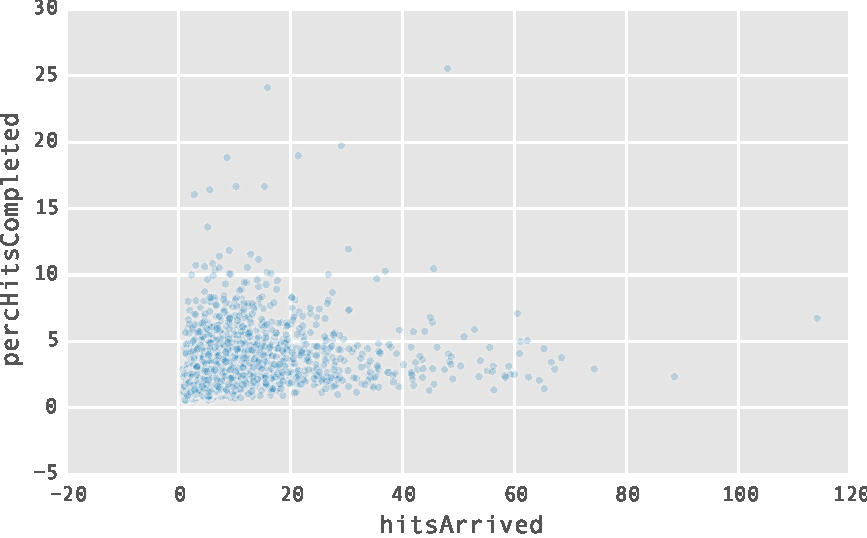
\includegraphics[width=0.5\textwidth]{figures/percHitsCompleted}
	\caption{The effect of new arrived HITs on the work provided supplied.}
	\label{fig:perc_hits_completed}
\end{figure}
Along the same lines, the results detailed in Figure\ref{fig:perc_hits_completed} indicate that as more HITs arrive, a higher percentage of the available work gets done. 
This clearly indicates that the arrival of new work also attracts new workers
in the market, who also seem to spillover to other tasks.

\begin{figure}[htbp]
	\centering
		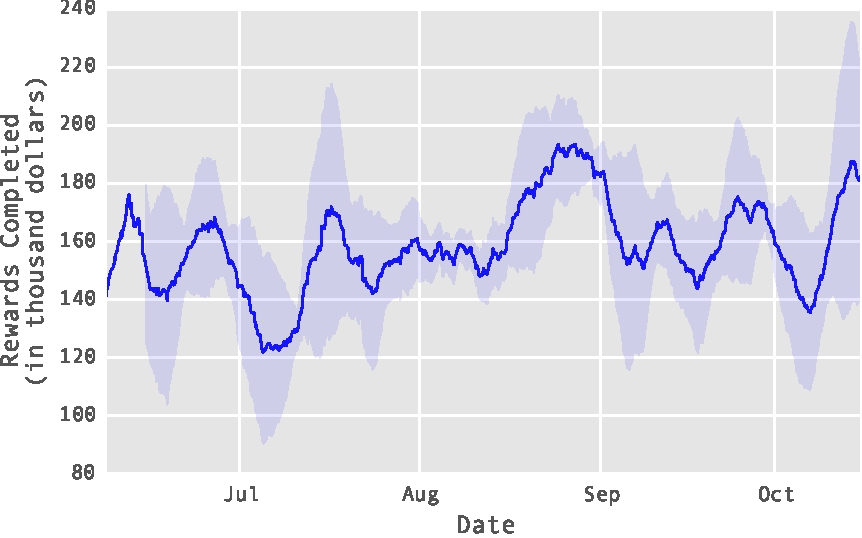
\includegraphics[width=0.5\textwidth]{figures/mac}
	\caption{MAC}
	\label{fig:mac}
\end{figure}
\begin{figure}[htbp]
	\centering
		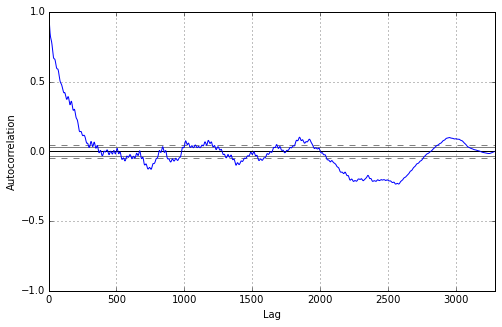
\includegraphics[width=0.5\textwidth]{figures/autocorrelation_plot}
	\caption{Autocorrelation  1}
	\label{fig:autocorrelation1}
\end{figure}
(Panos) It seems that there is significant memory for the market, as the autocorrelation of the 
HITS available (as reported by Amazon) lasts for approximately 7-10 days

\begin{figure}[htbp]
	\centering
		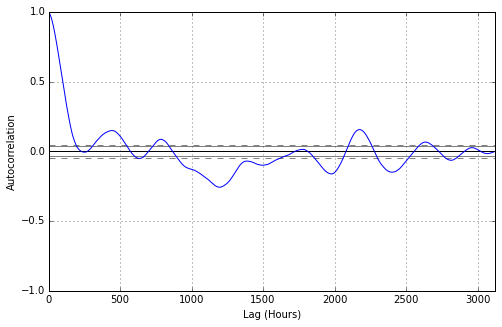
\includegraphics[width=0.5\textwidth]{figures/autocorrelation2}
	\caption{Autocorrelation 2}
	\label{fig:autocorrelation2}
\end{figure}

@Panos: The plot shows a strong weekly periodicity